
El diseño de estos instrumentales está enmarcado en el proyecto SOMA\cite{soma}, de Sistemas de OptoMecánica Abierta, del LEC. Este proyecto tiene como objetivos crear herramientas e instrumentos optomecánicos capaces de ser repetibles con facilidad y liberados a la comunidad. Libres en este contexto significa que el instrumental puede ser utilizado, adaptado o mejorado, y estos cambios pueden impactar en el proyecto, mejorando el resultado.

De esta forma, todos los diseños fueron efectuados con metodologías automatizadas, en particular los prototipos se hicieron con impresión 3D en plástico, además la electrónica utilizada es libre, y el software de adquisición de datos está hecho en plataformas de desarrollo y librerías libres.

\subsection{Perfilador}

El diseño y la tecnología necesaria para el funcionamiento del perfilador empezó a dilucidarse en Laboratorio 6, y para el final de Laboratorio 7 se reaplicó con éxito al polarimetro. Las partes mecánicas a diseñar y construir para el perfilador consistieron en el tambor, encargado de obturar el haz, el actuador o motor del tambor, que debió ser adquirido, y el soporte para el tambor y el motor.

En la figura \ref{fig:perfilador/esquema_bloques} se muestra un diagrama en bloques del perfilador, para tener noción de los componentes que representan y que partes fueron creadas

\begin{figure}[H]
    \centering
    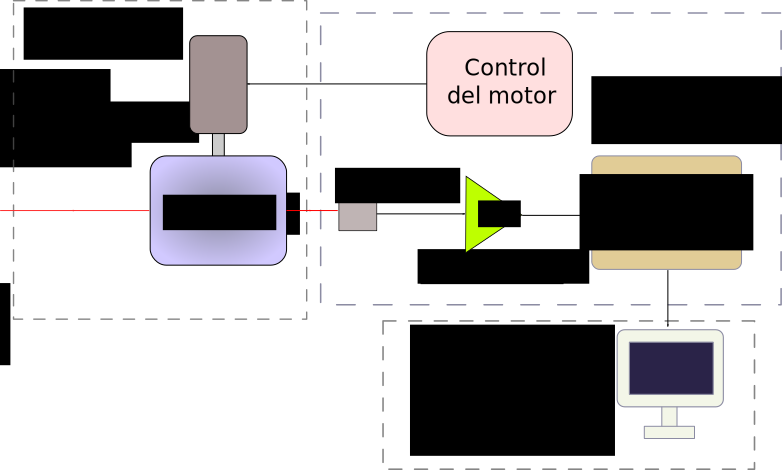
\includegraphics[width=0.5\textwidth]{fig/perfilador/esquema_bloques}
    \caption{Diagrama en bloques del perfilador construido}
    \label{fig:perfilador/esquema_bloques}
\end{figure}

El diseño de la electrónica y la adquisición de los datos se trata en un apartado aparte ya que tiene directa aplicación al polarimetro, además del perfilador.

\subsubsection{Tambor}
Como la velocidad objetivo de tambor (recordemos que esta velocidad permite una cinemática suave de adquisición) es de 24RPS, no se consideró, a priori, hacer un análisis del material a utilizar. Esto se justifica considerando que aún cuando la velocidad objetivo es de 1440RPM, es una velocidad bastante inferior a la velocidad de los  motores de alterna, que giran a 3000RPM, y las piezas de plástico impresas se saben que mantienen la estructura intacta a esas velocidades. De esta forma se construyó en plástico, con la impresora 3D, el tambor y se observó experimentalmente su funcionamiento.

El primer diseño, y único diseño salvo cambios de dimensiones, del tambor, consistió en un cilindro macizo de 15$\,$cm de diámetro, con un corte perpendicular al eje, hasta 5$\,$mm después de cruzar el eje, como se ve en la figura \ref{fig:perfilador/tambor}. Esto permite al girar el tambor ir cortando el haz, como se ve en la figura \ref{fig:perfilador/corte_tambor}, en este caso con un diámetro de hasta 10$\,$mm. 


\begin{figure}[H]
    \begin{subfigure}[b]{0.5\textwidth}
        \centering
        \includegraphics[width=0.3\textwidth]{fig/perfilador/tambor}
        \caption{}
        \label{fig:perfilador/tambor}
    \end{subfigure}
    \begin{subfigure}[b]{0.5\textwidth}
        \centering
        \includegraphics[width=0.4\textwidth]{fig/perfilador/corte_tambor}
        \caption{Esquema de la obturación}
        \label{fig:perfilador/corte_tambor}
    \end{subfigure}
    \caption{Tambor del perfilador}
\end{figure}

Este diseño permite que el tambor pueda entrar en compartimientos pequeños, y en particular se busca que el tambor entre en el interior de un sistema Cage Ø1'' de Thorlabs \cite{thorlabs_cage}; el sistema Cage representa uno de los entornos de trabajo más usuales del laboratorio, por lo que es necesario adaptar el perfilador a este.

La necesidad de usar una prolongación para obturar en vez de una ranura es producto de una decisión de diseño. Si el tambor con ranuras está entre el sensor y la fuente del haz, el sensor va a observar una obturación errónea, ya que el el haz va a ser obturado por la ranura de entrada del tambor y la ranura de salida, como se ve diagramado en la figura \ref{fig:perfilador/tambor_ranuras}. Debido a esto, es necesario obturar con la prolongación.

No solo eso, la prolongación permite obturar el haz hasta 4 veces por vuelta, dos veces dos planos diferentes del haz. Esto a su vez permitiría medir la divergencia, si es el haz diverge de forma apreciable en el diámetro de cilindroi, y también permite promediar dos obturaciones por plano en una vuelta. 

\begin{figure}[H]
\centering
\includegraphics[width=0.2\textwidth]{fig/perfilador/tambor_ranuras}
\caption{Corte transversal de un tambor con ranuras, donde se observar la ranura obturando un haz.}
\label{fig:perfilador/tambor_ranuras}
\end{figure}

Sin embargo, debe considerarse que la prolongación puede traer problemas mecánicos al rotar muy rápido, como ser una precesión al rotar o movimientos erráticos de la prolongación, que pueden producir mediciones del perfil erróneas. Por eso es de vital importancia medir el perfil del haz, en ambos planos de obturación, con otro perfilador, para calibrarlo correctamente.

También se construyó este diseño del tambor en aluminio, que tiene como ventaja menos oscilaciones al rotar y además tiene un filo más definido, pero lo que obtura el haz de forma más precisa. Sin embargo, la diferencia en tiempo de fabricación del tambor no justifica la mejora mecánica y además se necesita hacerle un proceso de galvanizado para no reflejar el haz al ambiente.


\subsubsection{Motor}

La velocidad de tambor debe ser tal que permita al perfilador generar una presentación de las mediciones con cinemática suave, que se logra adquiriendo y presentando con un refresco de 24 veces por segundo. Esto implica que el motor debe girar como mínimo a 24RPS (o 1440RPM).

Con esa premisa, se probaron todos los tipos de motores de corriente continua del mercado. Los motores de corriente altera y trifásicos se descartaron ya que no existen modelos de pequeñas dimensiones y exigen muchas precauciones eléctricas para su uso en una mesa óptica.

Como solución se eligieron los motores paso a paso. Un motor paso a paso corresponde a un motor de continua con un estator dentado con dos o más fases, como se ve en la figura \ref{fig:stepper_inner}. Al activar y desactivar en una secuencia la corriente por las fases se logra mover el rotor solamente un diente del estator o, lo que se denomina, un paso. Respecto a otros motores de continua tiene la ventaja de bloquearse si se pierde el sincronismo entre el rotor y el campo inducido, por lo que mantienen la velocidad de forma constante. Aún así pueden saltearse pasos si el torque a efectuar es muy grande, y con ello traería un problema en la medición. 

\begin{figure}[H]
    \begin{subfigure}[b]{0.33\textwidth}
        \centering
        \includegraphics[width=\textwidth]{fig/motor/diagrama_stepper}
        \caption{Esquema del motor paso a paso}
        \label{fig:stepper_inner}
    \end{subfigure}
    \begin{subfigure}[b]{0.33\textwidth}
        \centering
        \includegraphics[width=0.7\textwidth]{fig/motor/nema17}
        \caption{Motor NEMA 17}
    \end{subfigure}
    \begin{subfigure}[b]{0.33\textwidth}
    \centering
        \includegraphics[width=0.7\textwidth]{fig/motor/nema8}
        \caption{Motor NEMA 8}
    \end{subfigure}
    \caption{Esquema e imagenes de los motores paso a paso utilizados. El eje de ambos motores tienen un largo de mide 24$\,$mm, lo que dislumbra la diferencia en tamaño.}
\end{figure}
El motor paso a paso inicialmente adquirido corresponde al 42BYGHW609\cite{42BYGHW609}, con 200 pasos por vuelta y un torque de funcionamiento de 4$\,$kg$\,$cm. Este motor tiene la denominación NEMA 17, que determina el tamaño, 42,3$\times$42,3$\times$40$\,$mm, del motor y la ubicación de los agujeros de soporte. En la hoja de datos se observa que, en régimen de trabajo, se puede alcanzar una velocidad de 3000 pasos por segundo, es decir a 15RPS, con un torque de funcionamiento de 3kg$\,$cm; aún cuando esta información debe ser verificada experimentalmente, esto indica que el motor puede llegar a alcanzar las velocidades objetivo. 

El motor para alcanzar velocidades superiores a 10RPS necesita una aceleración constante, ya que debe cambiar el estado de movimiento de la inercia del eje y lo que tenga adosado en dicho. La electrónica de control, que es la misma que de adquisición, resuelve eso alterando la frecuencia de los pasos hasta llegar a la velocidad objetivo.

Después de efectuar pruebas y mediciones preliminarnes, en Laboratorio 6 principalmente, con el motor NEMA 17, se adquirió un motor NEMA 8, modelo 8H2A28402\cite{8H2A28402}, con dimensiones 20$\times$20$\times$28$\,$mm y 200 pasos por vuelta, como el modelo anteriormente utilizado. Este motor se logró hacerlo girar a 30RPS, con un cambio de la electrónica de control involucrada, y a esa velocidad pudo mover el tambor de plástico así como el de metal. De esta forma el motor rota más rápdido que la velocidad necesaria originalmente, sobrepasando las expectativas. Este motor también requiere de una aceleración menor para alcanzar altas velocidades, pero al tener menor inercia se alcanzó con mayores aceleraciones la velocidad final. Esto conlleva a menores tiempos en arrancar a medir y además menores tiempos muertos.



Este motor, al tener la mitad de tamaño en cada dimensión, permite diseñar un soporte que sea más fácil de integrar y medir en setups con limitaciones más importantes de espacio, además de achicar gastos en producción del soporte.

\subsubsection{Soporte}

El soporte del motor, el cuerpo principal del perfilador, fue diseñado considerando los setups usuales del laboratorio y la premisa básica de no desarmar ninguna estructura del experimento. 

El primer prototipo, que se ve en la figura \ref{fig:perfilador/soporte_v1}, usa el motor NEMA 17 y entra en el sistema óptico paralelo al plano óptico, es decir por un costado del setup. Este soporte a su vez tiene un agujero donde descansa el sensor, a 50$\,$mm de la mesa óptica (que representa la altura usual del laboratorio), y puede pegarse una lente con una distancia focal como máxima de 10$\,$mm para adaptarse para haces más grandes. En el costado tiene agujeros para ajustar el motor. Con el motor atornillado el prototipo tiende a caerse, por lo que es necesario ajustarlo a la mesa óptica. Este soporte no es autoportante.

\begin{figure}[H]
\centering
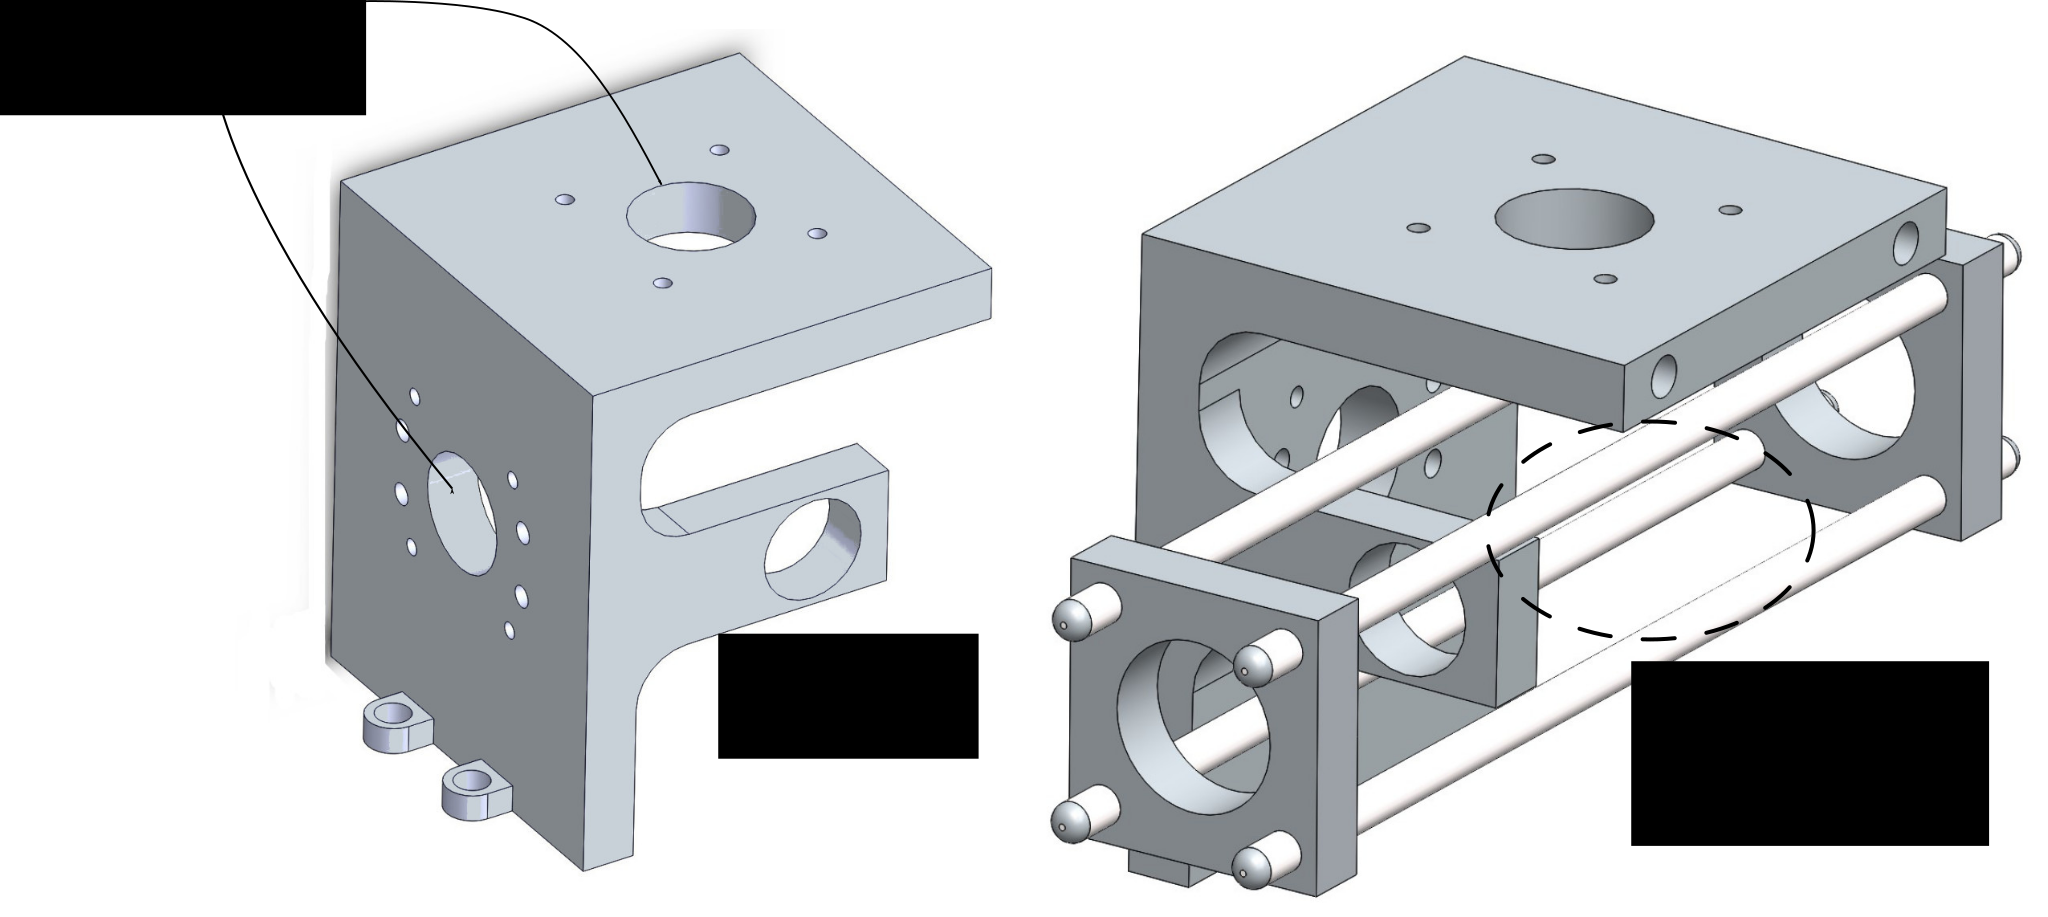
\includegraphics[width=0.55\textwidth]{fig/perfilador/soporte_v1}
\caption{Vista 3D del primer prototipo del soporte, junto con en ensamble en un posible Cage.}
\label{fig:perfilador/soporte_v1}
\end{figure}

Los agujeros de más en el plano izquierdo permiten atornillarlo al soporte de poste de Thorlabs, pero este diseño en esa situación solo permite perfilar en sólo eje.

El segundo prototipo, también con el motor NEMA 17, consiste en un un diseño autoportante como se ve en la figura \ref{fig:perfilador/soporte_v2}. Este soporte entra al plano óptico perpendicular a este, es decir por arriba de la mesa óptica.

\begin{figure}[H]
\centering
\includegraphics[width=0.65\textwidth]{fig/perfilador/soporte_v2}
\caption{Vistas tridimensionales del soporte, con el ensamble en un posible Cage.}
\label{fig:perfilador/soporte_v2}
\end{figure}

Este diseño tiene la ventaja soportar el motor sin la necesidad de ser atornillado y de poder medir en ambos ejes al estar adosado al soporte para postes de Thorlabs.

Ningún agujero tiene rosca, y además se los hicieron pasantes para los tornillos a utilizar; esto se debe a los límites impuestos por la impresora 3D utilizada. La mayoría del los agujeros tienen hasta 1$\,$mm más de diámetro para resultar pasantes en la impresión.

Habiendo hecho mediciones con ambos soportes, se llegó a la conclusión que el motor necesita estar encastrado para no generar problemas mecánicos en la medición. De esta forma el tercer prototipo del soporte, visto en la figura \ref{fig:perfilador/soporte_v3}, dispone de un encastre para el motor y además permite una muy rápida colocación en la mesa óptica. El sensor nuevamente descanza a 50$\,$mm de la mesa, y el largo de la prolongación permite medir correctamente cerca de un riel o en un Cage.

\begin{figure}[H]
\centering
\includegraphics[width=0.45\textwidth]{fig/perfilador/soporte_v3}
\caption{Vistas tridimensionales del soporte, con el ensamble en un posible Cage}
\label{fig:perfilador/soporte_v3}
\end{figure}

La desventaja de este soporte es la dificultado, y hasta imposibilidad por el tamaño del motor, usarlo en altura o poder medir en otro eje. De esta forma se diseño un modelo, visible en la figura \ref{fig:perfilador/soporte_v4}, alrededor de del motor NEMA 8 

\begin{figure}[H]
    \centering
    \includegraphics[width=0.35\textwidth]{fig/perfilador/soporte_v4}
    \caption{Vistas tridimensionales del soporte más el tambor de referencia}
    \label{fig:perfilador/soporte_v4}
\end{figure}

Este soporte tiene las ventajas de la anterior prototipo, como ser fácil colocación en la mesa óptica y con el motor encastrado para no tener mediciones erroneas. A su vez con un tornillo pasante en el centro del soporte es fácil de atornillar a cualquier soporte en altura o perpendicular para hacer mediciones en otros setups. El tamaño lateral al eje del motor está determinado por el tamaño del tambor, y por el tamaño del fotodiodo, pero se puede todavía achicar más en iteraciones siguientes.

\subsection{Electrónica de adquisición}

Como se busca al sistema lo más autónomo posible,  se necesita tener una electrónica con capacidad de mover el motor y medir el sensor de forma simultánea, y finalmente transmitir lo medido a una computadora. Esto implica que debemos construir un sistema embebido, y la mejor opción, si no la única viable, es utilizar un microcontrolador. 

\subsubsection{Controlador del motor}
Respecto al movimiento del motor, se utilizó un circuito integrado Pololu A4988\cite{pololu}, basado en Allegro A4988, que permite mover motores hasta 1$\,$A por fase y ejecutar pasos separados mínimamente por 1$\,\mu$s, más de lo necesario para el motor elegido, ya que representa una velocidad de rotación de 500RPS. Este integrado resuelve el control de corriente de las fases del motor, independiente de la tensión de la fuente. Es más permite setear el umbral de la corriente por un potenciometro, para aumentar el torque en caso de hacer microstepping, es decir mover el motor una fracción del paso. Como limitación a la tensión de entrada se necesita un mínimo de 8V, pero no es una limitación muy fuerte sobre la fuente; se usa una fuente de notebook de 19V con una corriente de  2A, a la cual no fue necesario filtrarla.

\subsubsection{Microcontrolador}
Respecto al microcontrlador, el laboratorio tenía disponible una placa Arduino\cite{arduino} UNO, que permite resolver la programación y la integración en proyectos de robótica o embebidos de forma simple para el usuario; se programa por USB y tiene un lenguaje de programación de alto nivel, en este caso un subconjunto de C++, y muchas librerías creadas por la comunidad para diversas aplicaciones.

Lamentablemente al mover el motor paso a paso y adquirir la señal analógica del fotodiodo al mismo, se encontró una limitación importante en la memoria RAM del Arduino UNO, de 2KiB. Este tamaño de memoria no es suficiente para guardar los datos de una vuelta, ya que solo se pudo guardar hasta 128 puntos (en este caso tiempo en microsegundos y tensión en bits del ADC), y se necesita guardar como mínimo 200 puntos o más si se usa microstepping. Es necesario medir una vez por paso, ya que de esta forma se tiene un disparo o trigger razonable para la adquisición analógica. 

Obviamente, se podría haber optado por medir 128 datos, pero al observar la transición para el haz de prueba se concluyó que esa cantidad de datos era insuficiente para conmensurar la transición con la precisión buscada; en este caso se observan 5 datos en una transición de un motor girando a 10RPS.

En la primera aproximación al control del motor, al transmitir los datos adquiridos se bloqueaba el movimiento del motor, ya que el tiempo consumido en esta transmisión es mayor al tiempo entre pasos. Para resolver esto, se utilizó la funcionalidad de PWM, Pulse Width Modulation, que consiste en una señal cuadrada con ancho de pulso variable (que para esta aplicación se usó un ciclo de trabajo del 50\%), con una frecuencia fija. Esta señal está generada por las interrupciones del microcontrolador, y no son alteradas por la transmisión de datos por el puerto USB.

Sin embargo para el Arduino UNO no es fácil de asignar la frecuencia de trabajo del PWM en cada pin, para lo cual es necesario cambiar detalles internos del microcontrolador.

Debido a todas estas limitaciones, se buscó un microcontrolador con mayor velocidad y más memoria RAM compatible con la plataforma Arduino, ya que se requiere que sea fácil de programar.

La placa de desarrollo Teensy v3.2\cite{teensy} cumplía con todo lo pedido; este dispositivo tiene una velocidad de procesador por defecto de 72MHz, y alcanza 96MHz, y 64KiB de RAM, tal vez un poco sobredimensionado para la aplicación. El pinout, es decir la funcionalidad de cada pin, se ve en la figura \ref{fig:circuito/teensy}. Además la plataforma de desarrollo tiene disponible un mecanismo simple para alterar la frecuencia del PWM, permitiendo generar aceleraciones y alcanzar velocidades más altas del motor fácilmente.

Probando la transmisión por USB de este microcontrolador se llegó al límite de 1200 datos transmitidos cada 0,5s. Este límite está impuesto por la velocidad de microcontrolador y la computadora utilizada, ya que el protocolo de transmisión está hecho por software.

Para aún mejorar más la portabilidad del instrumental, se buscó un integrado capaz de transmitir por radiofrecuencia, en especial WiFi ya que el protocolo TCP, el protocolo usando en redes de computadoras, maneja de forma eficiente paquetes grandes y puede mejorar aún más la velocidad de transferencia de datos.

El primer integradro con WiFi probado se denomina NodeMCU, que tiene la particularidad de ser programable por lenguajes de alto nivel, como es Lua o Python. Lamentablemente este integrado no tiene la velocidad de adquisición de datos necesaria, además de tener una documentación pobre, por lo que fue rápidamente descartado.

Finalmente, se hicieron pruebas con el microcontrolador Particle Photon\cite{particle_photon} (de Particle.io), que se puede ver en la figura \ref{fig:circuito/photon} (junto al lado del pinout del $\mu$C Teensy para comparar rápidamente). Este microcontrolador tiene integrado un circuito Broadcom BCM43362, que probee WiFi clase b/g/n, con un microcontrolador Freescale STM32F205 ARM Cortex M3 a 120MHz, con 128KB de RAM; de esta forma es microcontrolador Teensy, con el doble de memoria RAM, más todo el circuito de comunicación WiFi. 

 Respecto a la programación, el microcontrolador se programa en C++ enteramente, lo que hace mucho más simple el uso de librerías y código fuente de la comunidad. No solo eso, el sistema puede, y además se recomienda, ser programado desde Internet y además permite con una interfaz simple de usar publicar datos medidos en la nube cada 1s. Este microcontrolador está especialmente pensando para la Internet of Things, que busca automatizar y medir todos los procesos de los diferentes aparatos en una casa o en una oficina (como el aire acondicionado, la heladera, etc).

\begin{figure}[H]
    \begin{subfigure}[t]{0.5\textwidth}
        \centering
        \includegraphics[width=0.7\textwidth]{fig/circuito/teensy32_front_pinout}
        \caption{Pinout del $\mu$C Teensy}
        \label{fig:circuito/teensy}
    \end{subfigure}
    \begin{subfigure}[t]{0.5\textwidth}
        \centering
        \includegraphics[width=0.6\textwidth]{fig/circuito/photon}
        \caption{Pinout del $\mu$C Photon}
        \label{fig:circuito/photon}
    \end{subfigure}
    \caption{Microcontroladores utilizados comparado en su capacidades de entradas/salidas}
\end{figure}

\subsubsection{Amplificación de la señal}

El sensor utilizado corresponde a un fotodiodo  FDS010\cite{fds010} de Thorlabs, que en su hoja de datos determinar que se debe polarizar en inversa y utilizar una resistencia de carga. Un fotodiodo es modelado como una fuente de corriente dependiente de la luz incidente, por lo que es necesario transformar esa salida en una tensión medible. También se constató que la capacitancia del fotodiodo utilizado no altere la medición; en particular, este fotodiodo es capaz de responder en el orden de los nanosegundos, por lo que permite utilizarlo sin problemas.

Sin embargo, si se mide la corriente del fotodiodo en una resistencia de carga se observa un desajuste de la función error a la señal medida, como se ve en la figura \ref{fig:circuito/desajuste}

\begin{figure}[H]
    \centering
    \includegraphics[width=0.5\textwidth]{fig/perfilador/labo6/fit_data_labo6_anotado}
    \caption{Medición de la tensión en una resistencia de carga producida por la corriente del fotodiodo al perfilar un haz}
    \label{fig:circuito/desajuste}
\end{figure}

Este problema proviene de la resistencia de carga utilizada, que debido que la corriente del fotodiodo es muy pequeña, debe ser de un valor razonablemente grande. Esto produce que el circuito se comporte como un filtro RC pasa bajos, por lo que al tener un cambio brusco en la intensidad de luz, la corriente no responderá igual de rápido (al perder componentes en frecuencia). 

Para solucionar esto, se propone la construcción de un amplificador de transimpedancia, es decir un amplificador de corriente en tensión, por medio de un amplificador operacional. Este integrado permite crear circuitos complejos con muy pocas componentes, la mayoría pasivos, como en este caso una resistencia en la rama de retroalimentación; en la figura \ref{fig:circuito/tia} se ve el esquema del amplificador

\begin{figure}[H]
    \centering
    \includegraphics[width=0.25\textwidth]{fig/circuito/amp/TIA}
    \caption{Esquema del amplificador de transimpedancia implementado}
    \label{fig:circuito/tia}
\end{figure}

El operacional utilizado es el LM358, que tiene la ventaja de poder funcionar con fuente simple. De esta forma no es necesario tener tensiones negativas, pero si uno observa la hoja de datos del integrado se encuentra que no es rail-to-rail. Es decir la tensión máxima de salida no llega a a excursionar hasta la tensión de alimentación y además no es posible obtener una señal de salida con valor nulo (igual a 0V).

Para calibrar este amplificador se lo alimenta con una señal cuadrada, en este caso de corriente, para observar la respuesta en frecuencia y una señal triangular para observar la linealidad del sistema. Estas calibraciones se disponen en la figura \ref{fig:circuito/amp/transicion_escalon} y \ref{fig:circuito/amp/rango_lineal}.

\begin{figure}[H]
    \begin{subfigure}[b]{0.5\textwidth}
        \centering
        \includegraphics[width=0.9\textwidth]{fig/circuito/amp/transicion_cuadrada}
        \caption{Respuesta al escalón}
        \label{fig:circuito/amp/transicion_escalon}
    \end{subfigure}
    \begin{subfigure}[b]{0.5\textwidth}
        \centering
        \includegraphics[width=0.9\textwidth]{fig/circuito/amp/rango_lineal}
        \caption{Respuesta a una señal lineal}
        \label{fig:circuito/amp/rango_lineal}
    \end{subfigure}
    \caption{Calibraciones del amplificador de transimpedancia implementado}
\end{figure}

De la figura \ref{fig:circuito/amp/transicion_escalon} se deduce que el \emph{slew rate}, o tiempo de reacción del integrado, es de 0,4$\,$V $\mu$s$^{-1}$, que es hasta 4 veces más rápido de lo necesario según lo que se observa en las mediciones preliminares. Aún a una velocidad de 30RPS las transiciones se harían a 0,2 $\,$V $\mu$s$^{-1}$, por lo que el amplificador operacional está sobredimensionado.

Respecto al rango lineal no es posible acusar corrientes muy grandes ni corrientes nulas, pero el rango lineal es bastante amplio para las mediciones. En general la corriente oscura imposibilita generar mediciones de corriente nula, lo que permite usar satisfactoriamente este amplificador para la aplicación.

Finalmente la adquisición que se logró con el amplificador está plasmada en la figura \ref{fig:circuito/amp/perfilacion_ajuste}, donde se puede observar que la señal es ajustada correctamente por la función error, detalle que se esperaba que sucediera, solucionando el problema para el cual el amplificador fue construido exitosamente

\begin{figure}[H]
    \centering
    \includegraphics[width=0.45\textwidth]{fig/perfilador/fit_data_plastico_subida}
    \caption{Señal del fotodiodo al perfilar amplificada, con un ajuste de la función error}
    \label{fig:circuito/amp/perfilacion_ajuste}
\end{figure}
Cabe destacar que al amplificar la señal, también se amplifica el ruido de esta y la corriente oscura del fotodiodo, aún cuando esta bastante pequeña ya que no está polarizado en inversa, lo que hace la señal (como se ve en la figura \ref{fig:circuito/amp/perfilacion_ajuste}) más ruidosa. Sin embargo, la relación señal ruido es más que satisfactoria para la aplicación.

\subsubsection{Software el microcontrolador}
El circuito final fue implementado una placa de 5x5$\,$cm, junto con una fuente reductora de tensión para alimentar al microcontrolador a partir de la tensión del fuente de notebook, lo que permite utilizarlo fácilmente en la mesa óptica del laboratorio. El esquemático y el circuito impreso están liberados para el uso de la comunidad en el proyecto SOMA, y se encuentran en el apéndice.

El software del microcontrolador ya está pensando para el perfilador y polarimetro, midiendo la señal del fotodiodo solo cuando la computadora le manda la señal (es decir por un disparo externo), de forma sincrónica utilizando un delay proporcional al tiempo entre pasos del motor. Finalmente se manda toda la señal por protocolo Telnet, que no es más que un mensaje TCP con el texto del mensaje (en este caso los datos). En este caso al conectarse el cliente Telnet, la computadora, el microcontrolador nota la conexión y empieza a mandar la señal, y al final cierra la conexión; de esta forma no es necesario mandar ninguna señal del inicio, solamente conectarse a con la IP y el puerto TCP con un cliente Telnet.

El microcontrolador es capaz de mandar hasta 4000 datos cada 0,1s aproximadamente, lo que la velocidad de adquisición queda totalmente determinada por el motor; 4000 datos representan 20 vueltas del motor, o 40 transiciones, por lo que la velocidad de transferencia de datos es de 200 vueltas por segundo.

\subsection{Adquisición de datos}

Ya definido y construido el circuito del perfilador, en la computadora es necesario definir el software para obtener los datos crudos de la medición del fotodiodo, y finalmente deducir información útil del perfil. 

Para determinar el tamaño del haz, se propuso ajustar los datos asumiendo que el perfil es gaussiano. Como la medición de la corriente del fotodiodo corresponde a la integral de la intensidad del haz, el ajuste por cuadrados mínimos será de una función error, representada en la figura \ref{fig:perfilador/err_function}, donde el ancho medio se corresponde con la mitad del tamaño del haz.

Para poder encontrar el tamaño del haz a partir de varias transiciones, que provienen de la medición efecutada por la electrónica, es necesario definir la sección del gráfico o ventana temporal donde ajustar la función error. Para eso, se procede a obtener una frecuencia característica a partir de una transformada de Fourier y luego se buscan los puntos más cercanos al valor medio de la señal, por medio de un filtro gaussiano para detección de bordes. Finalmente se ajusta la función error dentro de la ventana temporal definida por un cuarto del tiempo característico (la inversa de la frecuencia característica) centrada los puntos más cercanos al valor medio. 

Es rescatable que todo este algoritmo procede de forma automático, solo asumiendo que los datos tienen las transiciones esperadas, y en caso de no tener una señal de esa forma se acusa un error, del cual se recupera y sigue midiendo.

Respecto al polarimetro, se ajusta una función coseno cuadrado y si el ajuste es exitoso se obtiene el coeficiente $\alpha$ (ecuación \ref{eq:polarizacion/alpha}), con los valores máximos y minimos del ajuste. De esta forma el software del polarimetro es muchisimo más simple que la del perfilador, lo que permitió crearlo rápidamente.

Todo el programa de obtención de los datos del microcontrolador y el acondicionamiento de datos se programó con Python v3.5, usando librerías Numpy v1.10.1, Scipy v0.16.1, Pandas v0.17 y Matplotlib v1.5.0, aunque funciona en versiones anteriores de la rama v3.x de Python. Este entorno, con la documentación, es libre en su totalidad, y además el software implementado está documentado para su posterior uso. 

El programa final de adquisición se le construyó una interfaz gráfica para poder ser más fácil de utilizar. Esta interfaz fue creada en PyQT, y es de muy fácil portado a todos los sistemas operativos usuales.

\subsection{Polarimetro}

Con la electrónica de adquisición y control del motor desarrollado para el perfilador, se construyó un polarímetro utilizando el concepto visto en la figura \ref{fig:polarimetro/esquema}. Para ello se consideró utilizar unos engranajes, uno de ellos motorizado y otro con la lámina polarizadora, y un fotodiodo midiendo la intensidad que atravieza la lámina.

El soporte diseñado para los engranajes se puede observar en la figura \ref{fig:polarimetro/soporte}, junto con los engranajes en la figura \ref{fig:polarimetro/engranajes}. El polarimetro funciona rotando el engranaje menor y el engranaje mayor tiene la lámina polarizadora pegada o colocada dentro de eje de dicho. El fotodiodo tiene un soporte detrás de la pieza, midiendo la intensidad del haz que atravieza la lámina polarizadora.

\begin{figure}[H]
    \begin{subfigure}{0.5\textwidth}
        \centering
        \includegraphics[width=0.4\textwidth]{fig/polarimetro/soporte_all}
        \caption{Polarímetro armado, sin el motor ni el fotodiodo}
        \label{fig:polarimetro/soporte}
    \end{subfigure}
    \begin{subfigure}{0.5\textwidth}
        \centering
        \includegraphics[width=0.35\textwidth]{fig/polarimetro/engranajes}
        \caption{Engranajes}
        \label{fig:polarimetro/engranajes}
    \end{subfigure}
    \caption{Vistas tridimensionales del polarímetro}
\end{figure}

Debido a imperfecciones del movimiento, el engranaje grande puede salirse del soporte, por lo que se le agregó una arandela (impresa) para limitar el movimiento en esa dirección. 

Finalmente, luego de imprimirse se debieron hacer algunos ajustes para mejorar la mecánica, lijando las superficies rotante. Esto también se debe a que en las impresiones 3D siempre se agrega material de soporte para que no se deforme mientras se imprime la pieza.

Igualmente, los problemas mecánicos persisten, por lo que se baja la velocidad (aumentando el torque) a 10RPS. A esta velocidad los engranajes giran sin problemas de forma continua, y además no mella la velocidad de adquisición de polarización. Hay que recordar que aunque  se busca medir en tiempo real, con solamente superar al mecanismo manual, que puede tardar entre 5 a 10 minutos por medición, se considera una mejora importante.

El soporte no está pensando explicitamente pensando para ser ubicado en altura, pero al ser de pequeñas dimensiones es factible crear con elementos del laboratorio una base con altura arbitraria. Además el soporte puede entrar fácilmente en un Cage de Thorlabs.
